\documentclass[border=2pt]{standalone}
\usepackage{tikz}
\usetikzlibrary{quotes,angles}
\usepackage{amsmath}

\begin{document}

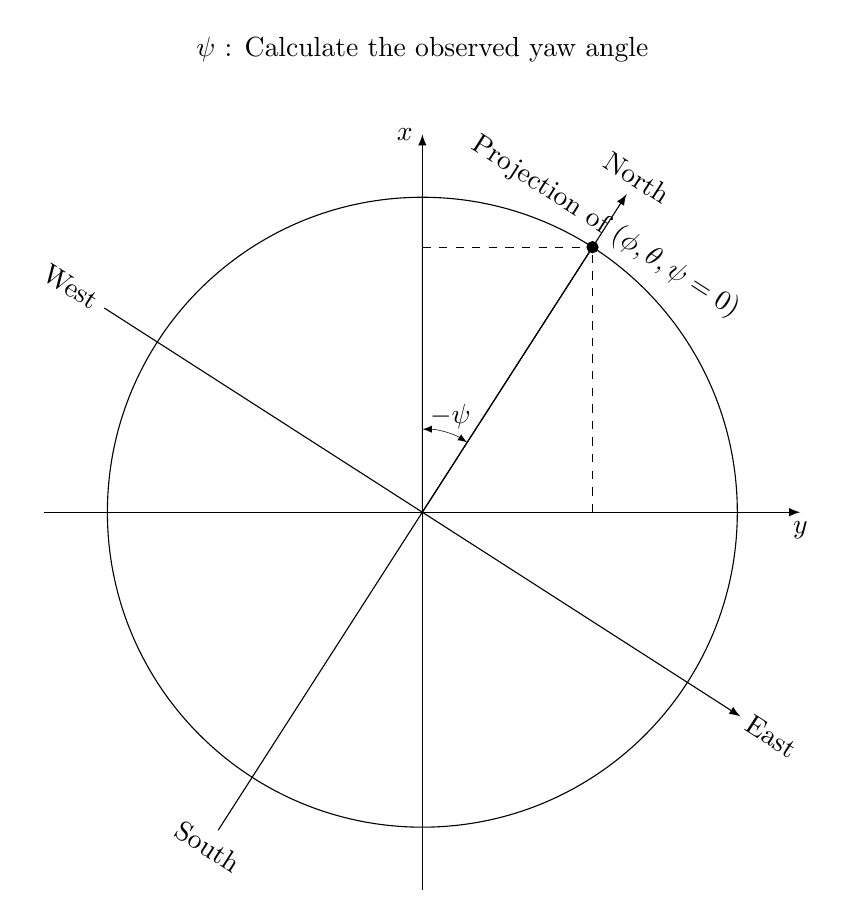
\begin{tikzpicture}[scale=4]

\node[above] at (0.0,1.40) {$\psi$ : Calculate the observed yaw angle};

% Draw x and y axis lines
\draw [->,>=latex] (-1.2,0) -- (1.2,0) node [below] {$y$};
\draw [->,>=latex] (0,-1.2) -- (0,1.2) node [left ] {$x$};

\begin{scope} [rotate=-32.7042]

\draw [->,>=latex] (-1.2,0) node [left , rotate=-32.7042] {West}  -- (1.2,0) node [right, rotate=-32.7042] {East};
\draw [->,>=latex] (0,-1.2) node [below, rotate=-32.7042] {South} -- (0,1.2) node [above, rotate=-32.7042] {North};
\node[above, rotate=-32.7042] at (0.0,1.0) {Projection of $\left(\phi,\theta,\psi=0\right)$};

\end{scope}

% Draw a circle at the origin of radius 1
\draw (0,0) circle (1);


\draw
  (0.5403,0.8415) coordinate (a) 
  -- (0,0) coordinate (b) 
  -- (0,1) coordinate (c) 
  pic["$-\psi$", draw=black, very thin, <->,>=latex, angle eccentricity=1.2, angle radius=30]
  {angle=a--b--c};

\draw [very thin, dashed] (0.5403,0) -- (0.5403,0.8415) ;
\draw [very thin, dashed] (0,0.8415) -- (0.5403,0.8415) ;
\filldraw[black] (0.5403,0.8415) circle (0.5pt) ;

\end{tikzpicture}

\end{document}

